\cleardoublepage
\chapter{Evaluation}\label{sec:eval}\minitoc\vspace{.5cm}
\index{Evaluation}\index{Validation}\index{Verification}

\section{Introduction}

\begin{wrapfigure}{r}{0.2\textwidth}
    \centering
    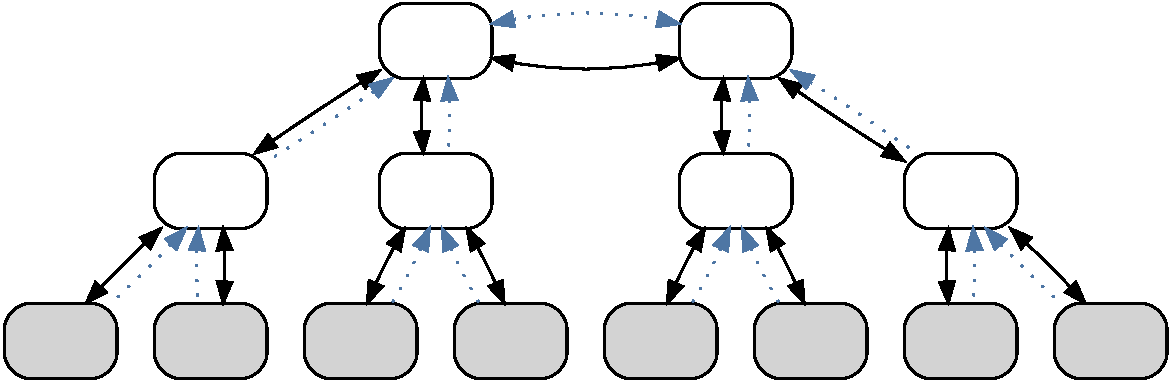
\includegraphics[width=0.2\textwidth]{resources/images/example3}
\end{wrapfigure}

\sidenote{Overview}
\todomid{write about \Cref{sec:eval:tec}}

\begin{figure}[htbp]
    \centering
    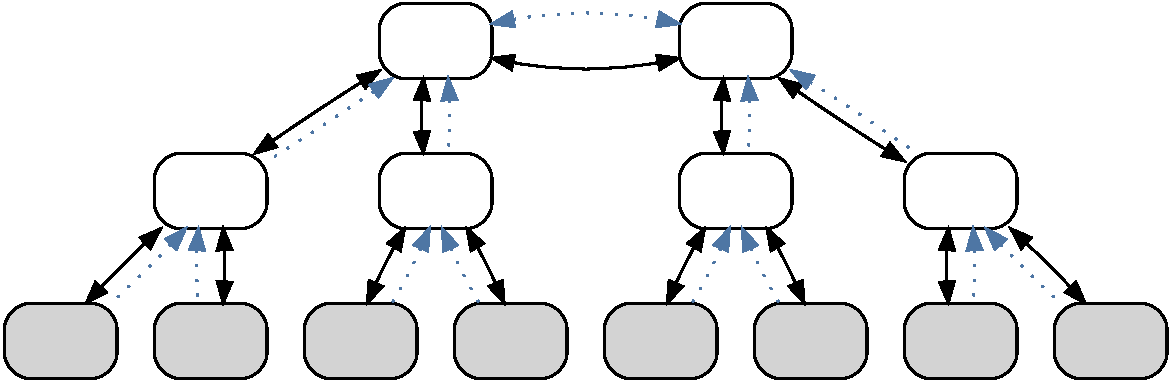
\includegraphics[width=.8\textwidth]{resources/images/example3}
    \caption{Choice of verification and validation techniques~\cite{li2002design}}\label{sec:eval:tec}
\end{figure}

\sidenote{Approaches}
\todomid{write}

\sidenote{Structure of Research}
\todomid{write about \Cref{fig:hourglass:evaluation}}

\begin{figure}[htpb]
    \centering
    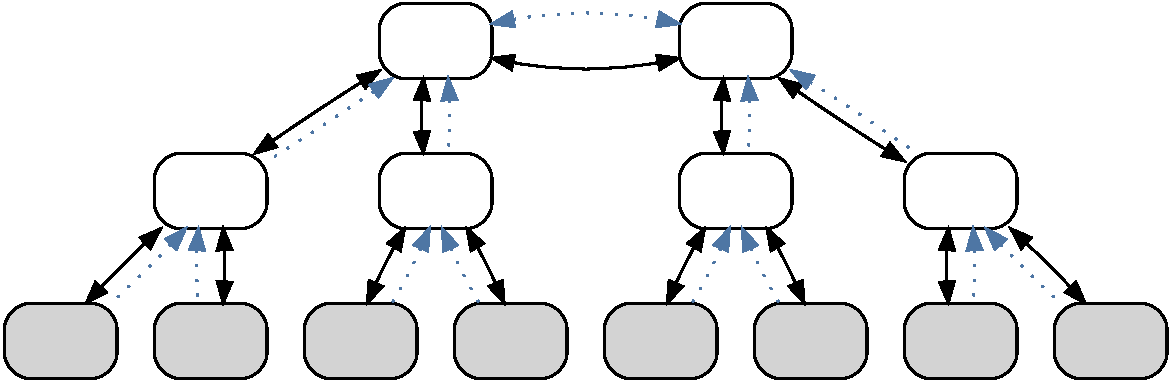
\includegraphics[width=.55\textwidth]{resources/images/example3}
    \caption{Placement of the evaluation in the structure of research}\label{fig:hourglass:evaluation}
\end{figure}

\section{Experimental Validation}

\sidenote{Overview}
\todomid{write about \Cref{tbl:eval:experiments}}

\begin{sidewaystable}
      \centering
      \captionsetup{type=table}
      \caption{Sideways table}
      \begin{tabular}{lllllll}\toprule
  \textbf{Experiment 1}   & \textbf{Experiment 2}  & \textbf{Experiment 3} & \textbf{Experiment 4} & \textbf{Experiment 5} & \textbf{Experiment 6} & \textbf{Experiment 7}  \\ \midrule
  CATCH & ME & IF & YOU & CAN & \emph{NOW} & OR NEVER \\
  CATCH & ME & IF & YOU & CAN & \emph{NOW} & OR NEVER \\
  CATCH & ME & IF & YOU & CAN & \emph{NOW} & OR NEVER \\
  CATCH & ME & IF & YOU & CAN & \emph{NOW} & OR NEVER \\
  CATCH & ME & IF & YOU & CAN & \emph{NOW} & OR NEVER \\
  CATCH & ME & IF & YOU & CAN & \emph{NOW} & OR NEVER \\
  CATCH & ME & IF & YOU & CAN & \emph{NOW} & OR NEVER \\
  CATCH & ME & IF & YOU & CAN & \emph{NOW} & OR NEVER \\
  CATCH & ME & IF & YOU & CAN & \emph{NOW} & OR NEVER \\
  CATCH & ME & IF & YOU & CAN & \emph{NOW} & OR NEVER \\
  CATCH & ME & IF & YOU & CAN & \emph{NOW} & OR NEVER \\
  \bottomrule
      \end{tabular}\label{tbl:eval:experiments}
\end{sidewaystable}


\subsection{Setup 1}

\sidenote{Overview}
\todomid{write}

\sidenote{Integration}
\todomid{write about \Cref{eq:var_idb}}

\small
\begin{equation}
  \begin{array}{l}
    \displaystyle t^{p_d}_{fw}(d) = \max_{d}(t_{child_{i}}) \\
    \displaystyle t^{p_d}_{db}(d) = \sum_{i=1}^{d} t_{db_{i}} \\
    \displaystyle t^{p_d}_{pc}(n,d) =
    	\begin{cases}
        	t_{pc}(d) + c(n) & \text{if $d = 1$,}\\
        	t_{pc}(d) + c(n) + \max(t_{avail}(d)) & \text{if $d>1$.}\\
        \end{cases}
  \end{array}\label{eq:var_idb}
\end{equation}
\normalsize

\sidenote{Example}
\todomid{write about \Cref{lst:eval:exp1}}

\needspace{5\baselineskip}\lstset{caption=Experiment 1, label=lst:eval:exp1,
language=ttl, breaklines=true, numbers=left,
stepnumber=1, frame=single, inputencoding=utf8/latin1}~\lstinputlisting{resources/code/example.java}

\subsection{Setup 2}

\sidenote{Overview}
\todomid{write}

\sidenote{Integration}
\todomid{write}

\sidenote{Example}
\todomid{write about \Cref{fig:eval:sub1,fig:eval:sub2,fig:eval:sub}}

\begin{figure}
    \begin{subfigure}[b]{.455\textwidth}
      \centering
      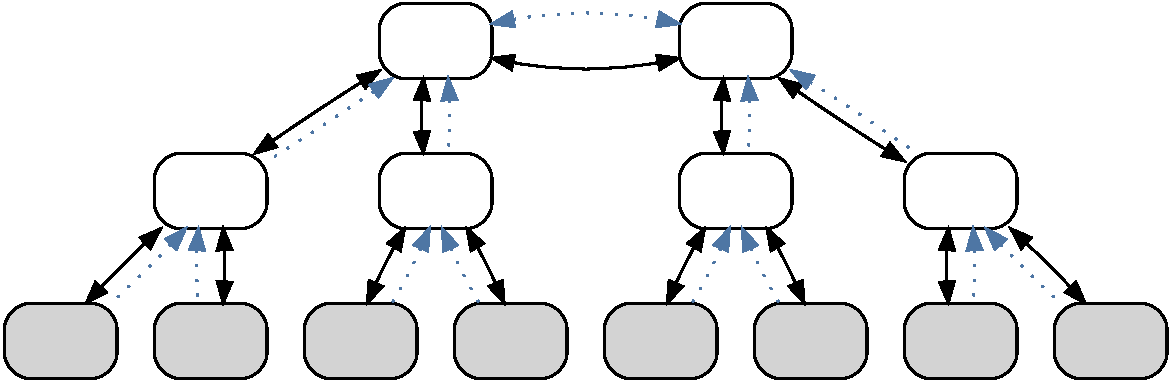
\includegraphics[width=.9\textwidth,frame]{resources/images/example3}
      \caption{Subfig 1}\label{fig:eval:sub1}
    \end{subfigure}~\begin{subfigure}[b]{.545\textwidth}
      \centering
      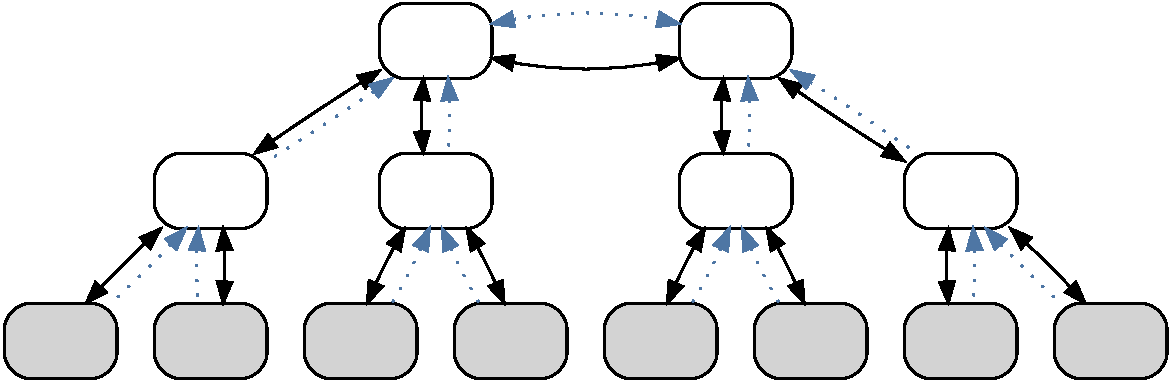
\includegraphics[width=1\textwidth,frame]{resources/images/example3}
      \caption{Subfig 2}\label{fig:eval:sub2}
    \end{subfigure}
    \caption{Sub Figures}\label{fig:eval:sub}
\end{figure}


\section{Performance Evaluation}

\sidenote{Overview}
\todomid{write}

\subsection{Evaluation 1}

\sidenote{Setup}
\todomid{write}

\sidenote{Cost Metrics}
\todomid{write}

\sidenote{Optimizing}
\todomid{write}

\sidenote{Performance Comparison}
\todomid{write}

\subsection{Evaluation 2}

\sidenote{Setup}
\todomid{write}

\sidenote{Response Times}
\todomid{write}
\begin{itemize}[noitemsep]
  \item \emph{In}: 159 ms $\pm$ 21 ms (95\% CI)
  \item \emph{Out}: 33 ms $\pm$ 5 ms (95\% CI)
  \item \emph{Between}: 238 ms $\pm$ 9 ms (95\% CI)
  \item \emph{After}: 45 ms $\pm$ 1 ms (95\% CI)
  \item \emph{Under}: 215 ms $\pm$ 2 ms (95\% CI)
  \item \emph{Over}: 148 ms $\pm$ 3 ms (95\% CI)
\end{itemize}

\sidenote{Scalability}
\todomid{write}

\section{Observational Validation}

\sidenote{Overview}
\todomid{write}

\subsection{Project 1}

\sidenote{Overview}
\todomid{write}

\sidenote{System Specification}
\todomid{write}

\sidenote{Extraction}
\todomid{write}

\sidenote{Example}
\todomid{write}

\subsection{Project 2}

\sidenote{Overview}
\todomid{write}

\sidenote{System Specification}
\todomid{write about \Cref{fig:eval:side}}

\begin{figure}[htbp]
    \centering
    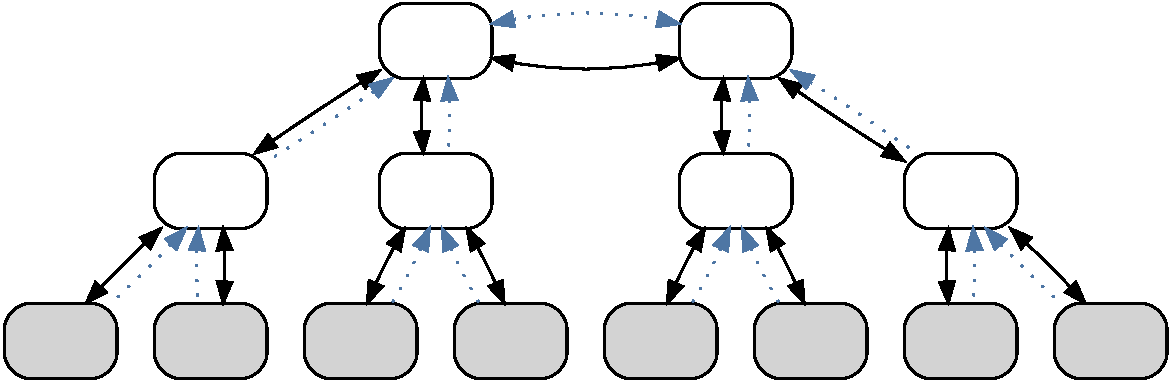
\includegraphics[height=.5\textwidth,angle=270]{resources/images/example3}
    \caption{Sideways figure}\label{fig:eval:side}
\end{figure}

\sidenote{Extraction}
\todomid{write}

\sidenote{Example}
\todomid{write}

\section{Deployments}

\sidenote{Overview}
\todomid{write}

\subsection{Installation 1}

\sidenote{Overview}
\todomid{write}

\sidenote{Integration}
\todomid{write}


\subsection{Installation 2}

\sidenote{Overview}
\todomid{write}

\sidenote{Integration}
\todomid{write}

\section{Code Verification}

\sidenote{Overview}
\todomid{write}

\sidenote{Static Tests}
\todomid{write}

\sidenote{Continuous Integration}
\todomid{write}

\sidenote{Test Coverage}
\todomid{write}

\section{Comparative Analysis}

\sidenote{Overview}
\todomid{write}

\subsection{Requirement Evaluation}

\sidenote{\Cref{tbl:reqs:compare}}
\todomid{write}

\begin{tabularx}{\textwidth}{p{2cm}X}
    \caption{Mapping requirements against own approach}\label{tbl:reqs:compare}\\
    \toprule
    \textbf{Requirements}& \textbf{Approach}  \\\midrule
    \endfirsthead%
    \toprule
    \textbf{Requirements}& \textbf{Approach}  \\\midrule
    \endhead%
\ref{req:stakeholder1:foo}\newline(Foo) &
\todomid{write}
\\\midrule

\ref{req:stakeholder1:bar}\newline(Bar) &
\todomid{write}
\\\midrule

\ref{req:stakeholder2:foo}\newline(Foo) &
\todomid{write}
\\\midrule

\ref{req:stakeholder2:bar}\newline(Bar) &
\todomid{write}
\\\midrule

\ref{req:stakeholder3:foo}\newline(Foo) &
\todomid{write}
\\\midrule

\ref{req:stakeholder3:bar}\newline(Bar) &
\todomid{write}

\\\bottomrule
\end{tabularx}

\subsection{Comparison with Other Approaches}

\sidenote{Overview}
\todomid{write}

\sidenote{\Cref{tbl:approaches:compare}}
\todomid{write about \Cref{tbl:approaches:compare}}

\begin{tabularx}{\textwidth}{p{2cm}LLLLLL}
    \caption{Comparison of related work with own approach}\label{tbl:approaches:compare}\\
    \toprule
    \textbf{Requirements} & \textbf{Related 1} & \textbf{Related 2} & \textbf{Related 3} & \textbf{Related 4} & \textbf{Related 5} & \textbf{Own Approach} \\\midrule
    \endfirsthead%
    \toprule
    \textbf{Requirements} & \textbf{Related 1} & \textbf{Related 2} & \textbf{Related 3} & \textbf{Related 4} & \textbf{Related 5} & \textbf{Own Approach} \\\midrule
    \endhead%

\ref{req:stakeholder1:foo}~\ref{req:stakeholder1:bar} & \textbf{(+)} & \textbf{(++)} & \textbf{(o)} & \textbf{(-)} & \textbf{(o)} & \textbf{(+++)} \\
(\ac{ABAC}) & \ac{ABAC} \ac{ABAC} v3, \ac{ABAC} \ac{ABAC} & \ac{ABAC} \ac{ABAC} v2, \ac{ABAC}, native \ac{ABAC} & \ac{ABAC} & native \ac{ABAC} & \ac{ABAC} \ac{ABAC} v2 & \ac{ABAC} \ac{ABAC} v3, \ac{ABAC} \ac{ABAC}, \ac{ABAC}, native \ac{ABAC}, native \\\midrule

\ref{req:stakeholder3:foo} & \textbf{(o)} & \textbf{(++)} &  & & \textbf{(++)} & \textbf{(+)} \\
(Details) & via foo & by bar / role-foo & --- & --- & bar / foo & foo-bar \\\midrule

\ref{req:stakeholder2:foo}~\ref{req:stakeholder2:bar}~\ref{req:stakeholder3:bar} & \textbf{(+)} & \textbf{(+)} & & \textbf{(+)} & \textbf{(+)} & \textbf{(+)} \\
(Barli) & via barli & via fooli & --- & via bar-foo & via foo-bar & via bar-bar \\\bottomrule
\end{tabularx}

\section{Conclusion}

\sidenote{Summary}
\todomid{write}

\sidenote{Takeaway 1}
\todomid{write}

\sidenote{Takeaway 2}
\todomid{write}

\sidenote{Takeaway 3}
\todomid{write}

\sidenote{Next chapter}
\todomid{write}
